\input /Users/davidmcallester/ICloude/tex/SlidePreamble
\input /Users/davidmcallester/ICloude/tex/preamble


\begin{document}

{\Huge

  \centerline{\bf TTIC 31230, Fundamentals of Deep Learning}
  \bigskip
  \centerline{David McAllester, Autumn 2020}
  \vfill
  \centerline{\bf Generative Adversarial Networks (GANs)}
\vfill
\vfill


\slide{Modeling Probability Distributions on Images}

Suppose we want to train a model of the probability distribution of natural images using cross-entropy loss.

\vfill
$$\Phi^* = \argmin_\Phi \;E_{y \sim \popd}\;-\ln p_\Phi(y)$$

\vfill
Images are continuous stuctured objects --- a continuous value at every pixel.

\vfill
It is difficult to build probability models for images (or other continuous structured values)
that both accurately model the distribution and also allow us to calculate $p_\Phi(y)$.

\slide{Generative Adversarial Networks (GANs)}

GANs represent $p_\Phi(y)$ implicitly by constructing an image generator and abandon the ability to compute $p_\Phi(y)$.

\vfill
The cross-entropy loss is replaced by an adversarial discriminator which tries to distinguish between generated images and real images.

\anaslide{Representing a Distribution with a Generator}

\bigskip
\centerline{$z$\hspace{5in}$y_\Phi(z)$}
\centerline{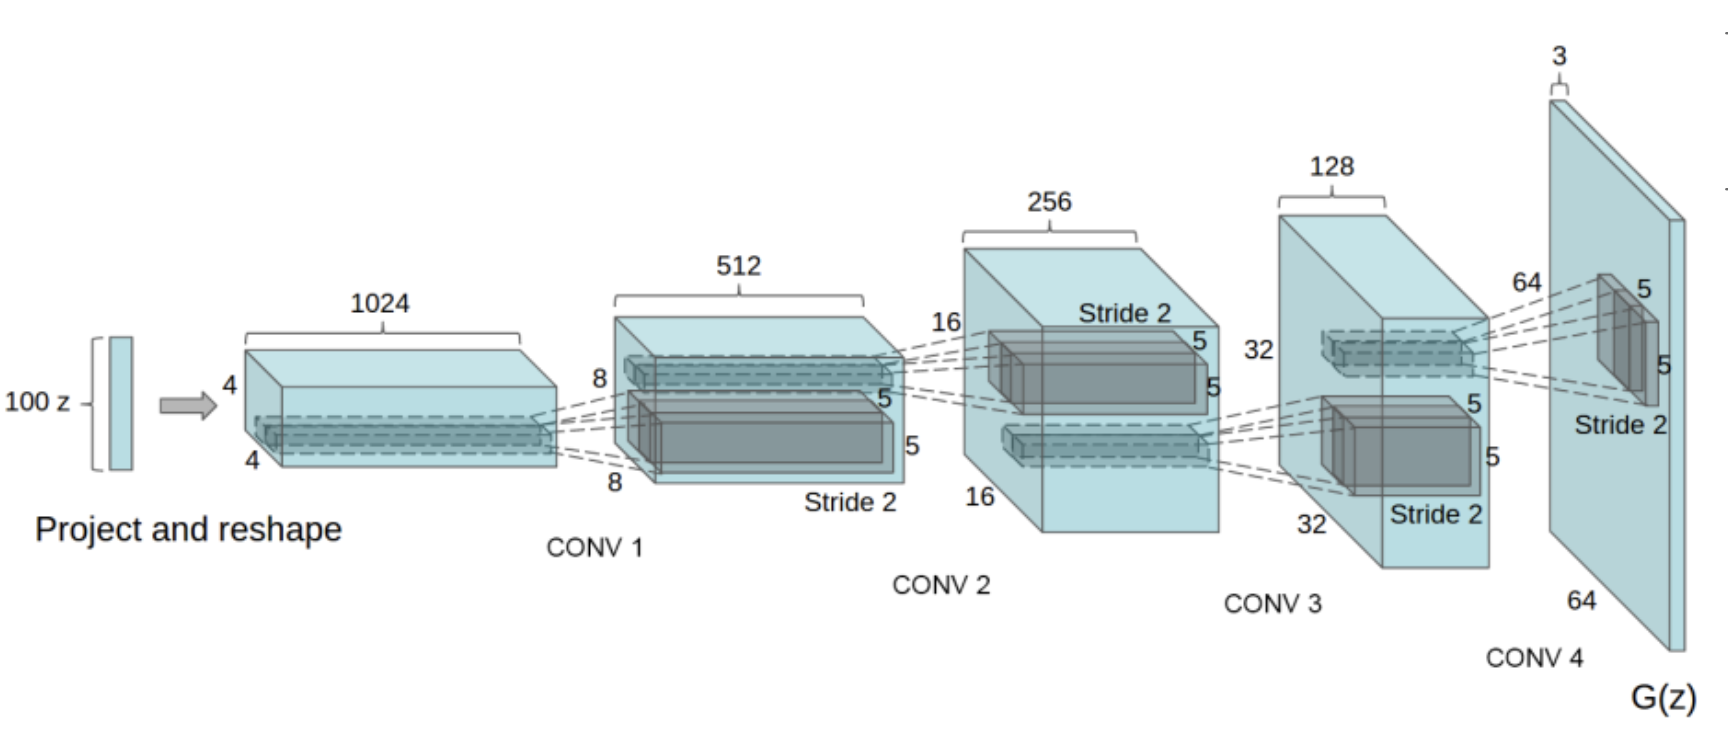
\includegraphics[width=6in]{\images/generator1}}

\bigskip
The random input $z$ defines a probability density on images $y_\Phi(z)$.  We will write this as $p_\Phi(y)$ for the image $y$.

\anaslide{Representing a Distribution with a Generator}

\bigskip
\centerline{$z$\hspace{5in}$y_\Phi(z)$}
\centerline{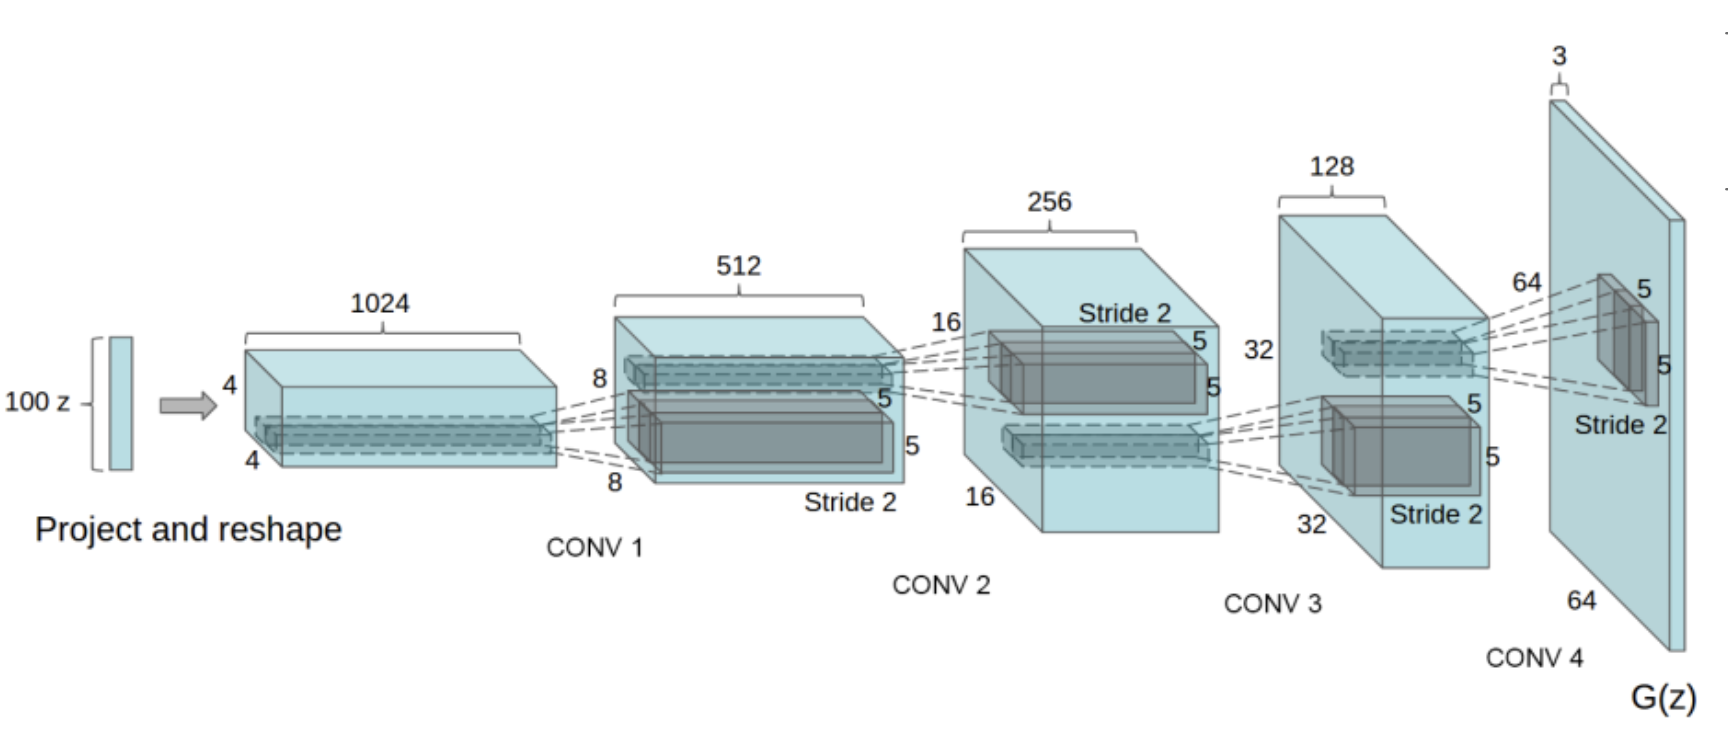
\includegraphics[width=6in]{\images/generator1}}

\bigskip
We want $p_\Phi(y)$ to model a natural image distribution such as the distribution over human faces.


\anaslide{Representing a Distribution with a Generator}

\bigskip
\centerline{$z$\hspace{5in}$y_\Phi(z)$}
\centerline{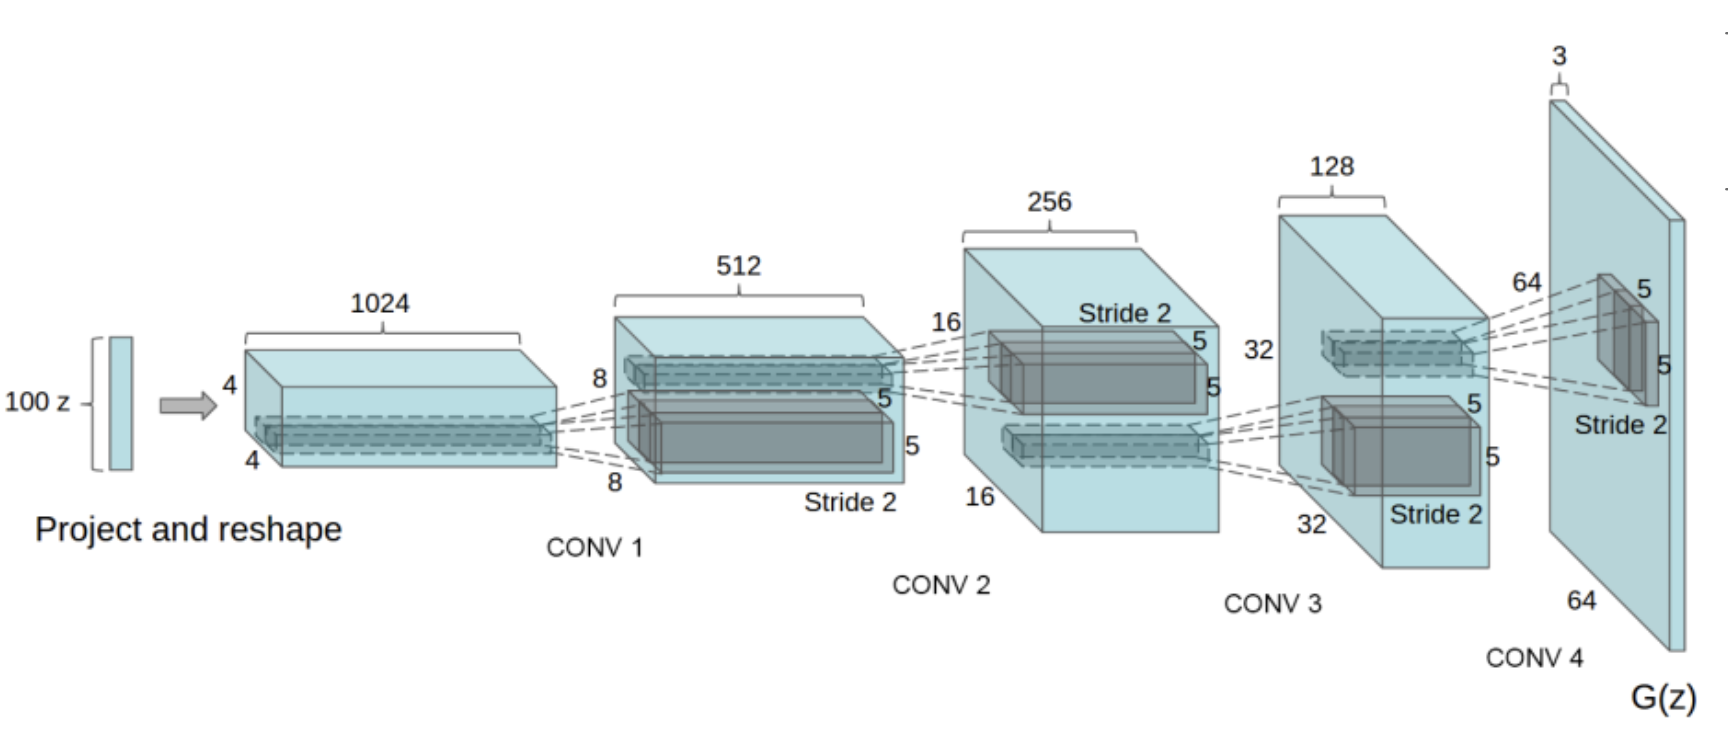
\includegraphics[width=6in]{\images/generator1}}

\bigskip
We can sample from $p_\Phi(y)$ by sampling $z$.  But we cannot compute $p_\Phi(y)$ for $y$ sampled from the population.

\slidetwo{Increasing Spatial Dimension}{(ConvTranspose in PyTorch)}

\centerline{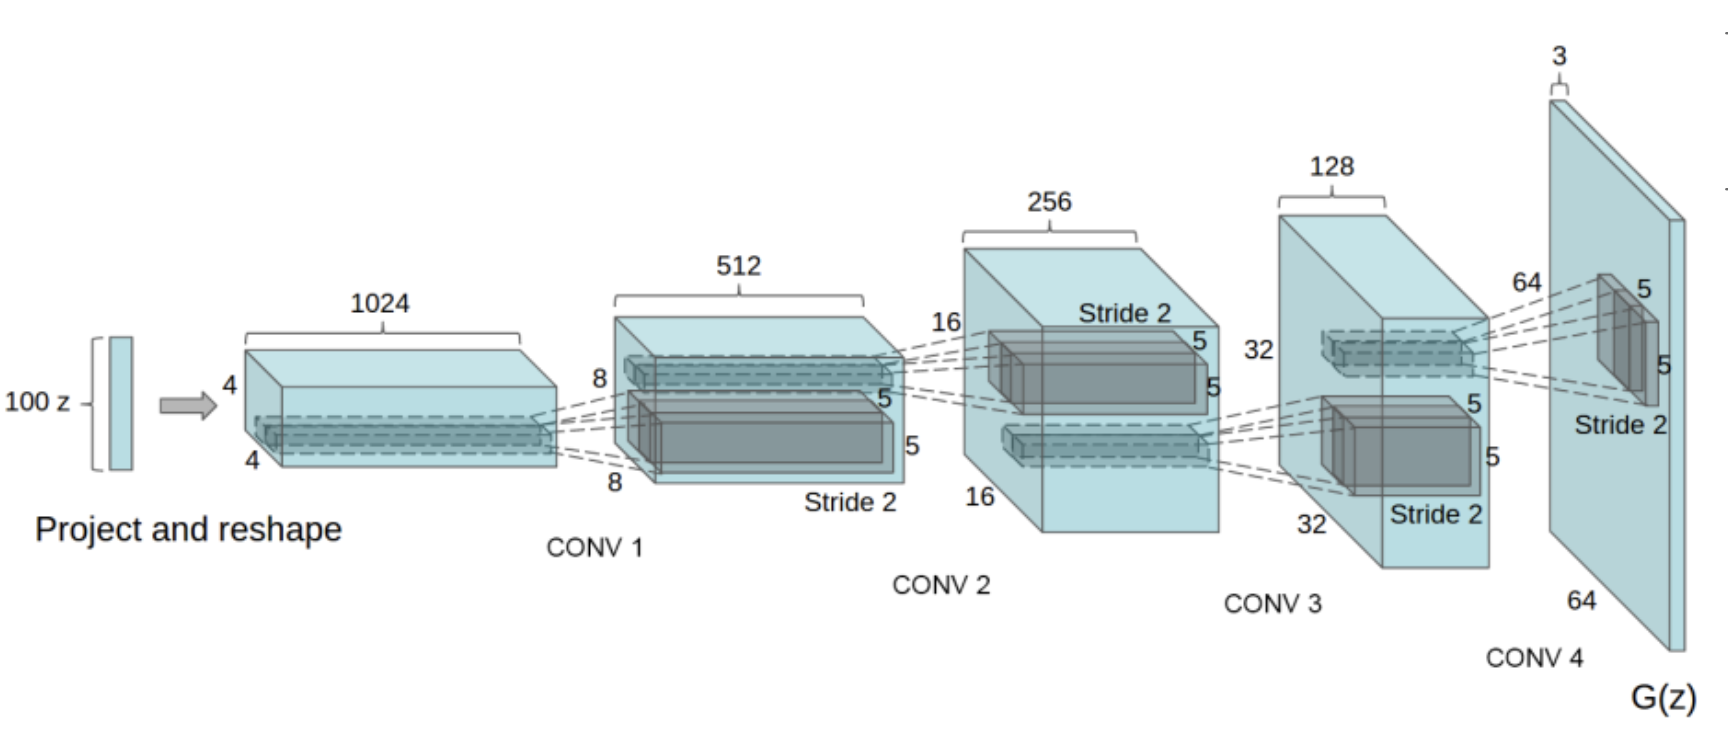
\includegraphics[width=5in]{\images/generator1}}

\vfill
To increase spatial dimension we use 4 times the desired number of output features.

\begin{eqnarray*}
  L'_{\ell+1}[x,y,i] & = & \sigma\left(W[\Delta X, \Delta Y, J,i]\; L'_\ell[x + \Delta X, y + \Delta Y, J]\right)
\end{eqnarray*}

\vfill
We then convert $L'_{\ell+1}[X,Y,I]$ to $L'_{\ell+1}[2X,2Y,I/4]$.

\slide{Generative Adversarial Networks (GANs)}

Let $y$ range over images.  We have a generator $p_\Phi$. For $i \in \{-1,1\}$ we define a probability distribution over pairs
$\tuple{i,y}$ by
\begin{eqnarray*}
\tilde{p}_\Phi(i = 1) & = & 1/2 \\
\tilde{p}_\Phi(y|i=1) & =&  \popd(y) \\
\tilde{p}_\Phi(y|i=-1) & = & p_\Phi(y)
\end{eqnarray*}

\vfill
We also have a discriminator $P_\Psi(i|y)$ that tries to determine the source $i$ given the image $y$.

\vfill
The generator tries to fool the discriminator.
\begin{eqnarray*}
\Phi^* & = & \argmax_\Phi\;\;\min_\Psi\;E_{\tuple{i,y} \sim \tilde{p}_\Phi}\;-\ln P_\Psi(i|y)
\end{eqnarray*}

\slide{GANs}

The generator tries to fool the discriminator.

\vfill
\begin{eqnarray*}
\Phi^* & = & \argmax_\Phi\;\;\min_\Psi\;E_{\tuple{i,y} \sim \tilde{p}_\Phi}\;-\ln P_\Psi(i|y)
\end{eqnarray*}

\vfill
Assuming universality of both the generator $p_\Phi$ and the discriminator $P_\Psi$ we have {\color{red} $p_{\Phi^*} = \popd$}.

\vfill
Note that this involves only discrete cross-entropy.

\slide{GANs}

To make the gradient descent clearer we write

\vfill
$$E_{\tuple{i,y} \sim \tilde{p}_\Phi}\;-\ln P_\Psi(i|y)$$

\vfill
as

\vfill
$$\frac{1}{2} E_{y \sim \popd}\;-\ln P_\Psi(1|y) \;\;\;+\;\;\; \frac{1}{2} E_{z \sim {\cal N}(0,I)}\;-\ln P_\Psi(-1|y_\Phi(z))$$

\slidetwo{Generative Adversarial Nets}{Goodfellow et al., June 2014}
\centerline{\includegraphics[width = 9in]{\images/GAN2014}}
The rightmost column (yellow boarders) gives the nearest neighbor in the training data to the adjacent column.

\slide{GAN Mode Collapse}

A major concern is ``mode collapse'' where the learned distribution omits a significant fraction of the population distribution.

\vfill
There is no quantitative performance measure that provides a meaningful guarantee against mode collapse.

\slide{The Fr\'{e}nchet Inception Score (FID)}

The main problem with GANs is the lack of a meaningful quantitative evaluation metric.

\vfill
A standard quantitative performance measure is French\'{e}t Inception Distance (FID).

\vfill
This measures statistics of the features
of the inception image classification model (trained on imagenet) for images generated by the generator.

\vfill
It then compares those statistics
to the same statistics for images drawn from the population.

\vfill
But the FID score provides no guarantees against mode collapse.

\slide{END}

}
\end{document}
